\documentclass{article}
\usepackage{amsmath,amsfonts,amsthm,amssymb,amsopn,bm}
\usepackage[margin=.9in]{geometry}
\usepackage{graphicx}
\usepackage{url}
\usepackage[usenames,dvipsnames]{color}
\usepackage{fancyhdr}
\usepackage{multirow}
\usepackage{listings}

\definecolor{keywords}{RGB}{255,0,90}
\definecolor{comments}{RGB}{0,0,113}
\definecolor{red}{RGB}{160,0,0}
\definecolor{green}{RGB}{0,150,0}
 
\lstset{language=Python, 
        basicstyle=\ttfamily\tiny, 
        keywordstyle=\color{keywords},
        commentstyle=\color{comments},
        stringstyle=\color{red},
        showstringspaces=false}

\newcommand{\field}[1]{\mathbb{#1}}
\newcommand{\1}{\mathbf{1}}
\newcommand{\E}{\mathbb{E}} 
\renewcommand{\P}{\mathbb{P}}
\newcommand{\R}{\field{R}} % real domain
% \newcommand{\C}{\field{C}} % complex domain
\newcommand{\F}{\field{F}} % functional domain
\newcommand{\T}{^{\textrm T}} % transpose
\def\diag{\text{diag}}

%% operator in linear algebra, functional analysis
\newcommand{\inner}[2]{#1\cdot #2}
\newcommand{\norm}[1]{\left\|#1\right\|}
\newcommand{\twonorm}[1]{\|#1\|_2^2}
% operator in functios, maps such as M: domain1 --> domain 2
\newcommand{\Map}[1]{\mathcal{#1}}
\renewcommand{\theenumi}{\alph{enumi}} 

\newcommand{\Perp}{\perp \! \! \! \perp}

\newcommand\independent{\protect\mathpalette{\protect\independenT}{\perp}}
\def\independenT#1#2{\mathrel{\rlap{$#1#2$}\mkern2mu{#1#2}}}
\newcommand{\vct}[1]{\boldsymbol{#1}} % vector
\newcommand{\mat}[1]{\boldsymbol{#1}} % matrix
\newcommand{\cst}[1]{\mathsf{#1}} % constant
\newcommand{\ProbOpr}[1]{\mathbb{#1}}
\newcommand{\points}[1]{\small\textcolor{magenta}{\emph{[#1 points]}} \normalsize}
\date{{}}

\setlength\parindent{0px}

\begin{document}
\title{Homework \#0 }
\author{\normalsize{Spring 2020, CSE 446/546: Machine Learning}\\
\normalsize{Dino Bektesevic}}
\maketitle


\section*{Probability and Statistics}
A.1 \points{2} (Bayes Rule, from Murphy exercise 2.4.) After your yearly checkup, the doctor has bad news and good news. The bad news is that you tested positive for a serious disease, and that the test is 99\% accurate (i.e., the probability of testing positive given that you have the disease is 0.99, as is the probability of testing negative given that you don't have the disease). The good news is that this is a rare disease, striking only one in 10,000 people. What are the chances that you actually have the disease? (Show your calculations as well as giving the final result.)\\

Denoting $X=1$ as test result being positive and $Y=1$ as actually having the disease, following Bayes rule we have
\begin{align*}
    P(Y=1|X=1) &= \frac{P(X=1|Y=1)P(Y=1)}{P(X=1|Y=1)+P(X=1|Y=0)P(Y=0)} \\
    &= \frac{0.99\cdot0.0001}{0.99\cdot0.0001 + 0.01*0.9999} \\
    &= 0.0098 \approx 1\%
\end{align*}
since we are given that $P(X=1|Y=1)=P(X=0|Y=0)=0.99$ and $P(Y=1)=1/10000=0.0001$ from which it follows that $P(Y=0)=1-P(Y=1)=0.9999$ and $P(X=1|Y=0)=1-P(X=0|Y=0)=0.01$
\newline
\newline
A.2 For any two random variables $X,Y$ the \emph{covariance} is defined as $\text{Cov}(X,Y)=\E[(X-\E[X])(Y-\E[Y])]$. You may assume $X$ and $Y$ take on a discrete values if you find that is easier to work with.
    \begin{enumerate}
         \item \points{1} If $\E[Y|X=x] = x$ show that $\text{Cov}(X,Y) = \E[(X-\E[X])^2]$. 
         Simplify the right hand side of the expression for covariance (marking expectation values that are scalars by replacing them with $\mu$ to show they can be taken out of expectation value operator):
             \begin{align*}
                 E[(X-E(X))^2] &= E[ X^2 - 2XE(X) + E(X)^2 ] = E[X^2 - 2\mu_xX + 2\mu_x^2] \\
                 &=E[X^2] - 2\mu_xE[X] + \mu_x^2 = =E[X^2] - 2\mu_x^2 + \mu_x^2 \\
                 &=E[X^2]-\E[X]^2 = \text{Var}(X)
             \end{align*}
         It's clear now that we are actually looking to show that $\text{Cov}(X,Y)=\text{Var}(X)$. Apply what is given in the problem to law of iterative expectations: 
             \begin{align*}
                 E[Y] = \int yp(y)dy = \int E(Y|X=x)p(x) dx = \int xp(x)dx = E[X]
             \end{align*}
         Finally, write out the expression for covariance of two rvs:
             \begin{align*}
                 \text{Cov}(X,Y) = E[XY] - E[X]E[Y] = E[XY] - E[X]^2 = \text{Var}(X)
             \end{align*}
         since we can write the joint probability $E[XY]=\int\int xp(x)yp_{Y|X=x}(y)dxdy = \int xp(x)x dx = \int x^2p(x)dx = E[X^2]$
         \item \points{1} If $X,Y$ are independent show that $\text{Cov}(X,Y)=0$.
             \begin{align*}
                 \text{Cov}(X,Y) = E(X,Y) - E(X)E(Y) = E(X)E(Y) - E(X)E(Y) = 0
             \end{align*}
\end{enumerate}

A.3 Let $X$ and $Y$ be independent random variables with PDFs given by $f$ and $g$, respectively. Let $h$ be the PDF of the random variable $Z = X+Y$.
\begin{enumerate}
	\item \points{2} Show that $h(z) = \int_{-\infty}^\infty f(x) g( z - x ) d x $.  (If you are more comfortable with discrete probabilities, you can instead derive an analogous expression for the discrete case,  and then you should give a one sentence explanation as to why your expression is analogous to the continuous case.).
	\item \points{1} If $X$ and $Y$ are both independent and uniformly distributed on $[0,1]$ (i.e. $f(x)=g(x)=1$ for $x \in [0,1]$ and $0$ otherwise) what is $h$, the PDF of $Z=X+Y$?
\end{enumerate}

A.4 \points{1} A random variable $X \sim \mathcal{N}(\mu, \sigma^2)$ is Gaussian distributed with mean $\mu$ and variance $\sigma^2$. Given that for any $a,b \in \R$, we have that $Y = aX + b$ is also Gaussian, find $a,b$ such that $Y \sim \mathcal{N}(0,1)$.
\begin{align*}
    E[Y] &= aE[X]+b = 0\\
    \text{Var}[Y] &= a^2\text{Var}[X] = 1\\
    a\mu + b &= 0\\
    a^2\sigma^2 &= 1\\
    a &= 1/\sigma\\
    b &= - \mu/\sigma\\
\end{align*}

A.5 \points{2} For a random variable $Z$, its mean and variance are defined as $\E[Z]$ and $\E[(Z-\E[Z])^2]$, respectively. Let $X_1,\dots,X_n$ be independent and identically distributed random variables, each with mean $\mu$ and variance $\sigma^2$. If we define $\widehat{\mu}_n = \frac{1}{n} \sum_{i=1}^n X_i$, what is the mean and variance of $\sqrt{n}(\widehat{\mu}_n - \mu)$? \\

The average value of many random i.i.d. variables that have the same mean $\mu$ is the mean $\mu$ itself. So :
$$\hat\mu_n = \frac{1}{n}\sum X_i = \mu$$
so:
$$\sqrt{n}(\hat\mu_n - \mu) = 0$$

The variance of many i.i.d. rvs can be written as:
\begin{align*}
    \text{Var}[\sqrt n \hat\mu_n - \sqrt n \mu] &= n\text{Var}[\hat\mu_n]+n\text{Var}[\mu] \\
    &= n \text{Var}[\hat\mu_n] = \frac{n\sigma^2}{n} = \sigma^2
\end{align*}
since $\text{Var}[aX]=a^2\text{Var}[X]$ and $\text{Var}[\mu]=0$ because all observed rvs have the same mean.\\

A.6 If $f(x)$ is a PDF, the cumulative distribution function (CDF) is  defined as $F(x) = \int_{-\infty}^x f(y) dy$.  For any function $g : \R \rightarrow \R$ and random variable $X$ with PDF $f(x)$, recall that the expected value of $g(X)$ is defined as $\E[g(X)] = \int_{-\infty}^\infty g(y) f(y) dy$. For a boolean event $A$, define $\1\{ A \}$ as $1$ if $A$ is true, and $0$ otherwise. Thus, $\1\{ x \leq a \}$ is $1$ whenever $x \leq a$ and
  $0$ whenever $x > a$.  Note that $F(x) = \E[\1\{X \leq x\}]$.  Let $X_1,\dots,X_n$ be \emph{independent and identically distributed} random variables with CDF $F(x)$.  Define $\widehat{F}_n(x) = \frac{1}{n} \sum_{i=1}^n \1\{X_i \leq x\}$. Note, for every $x$, that $\widehat{F}_n(x)$ is an \emph{empirical estimate} of  $F(x)$. You may use your answers to the previous problem. 
  \begin{enumerate}
  
  \item \points{1} For any $x$, what is $\E[ \widehat{F}_n(x) ]$?
  \begin{align*}
      E[\hat F_n(x)] &= E\left[ \frac{1}{n}\sum_{i=1}^n \mathbf{1} \left\{ X_i \leq x \right\} \right] \\
      &= \frac{1}{n}\sum_{i=1}^n E\left[\mathbf{1} \left\{ X_i \leq x \right\} \right] \\
      &= \frac{1}{n}\sum_{i=1}^n F(x) \\
      &= \frac{1}{n} n F(x) = F(x)
  \end{align*}  
  
  \item \points{1} For any $x$, the variance of $\widehat{F}_n(x)$ is $\E[ ( \widehat{F}_n(x) - F(x) )^2 ]$. Show that $\textrm{Variance}(\widehat{F}_n(x)) = \frac{F(x)(1-F(x))}{n}$. \\
  \begin{align*}
  {Var}\hat F_n(x) &= \text{Var} \frac{1}{n}\sum_{i=1}^n \mathbf{1} \left\{ X_i \leq x \right\} \\
      &= \frac{1}{n^2}\text{Var}\left(\sum_{i=1}^n \mathbf{1} \left\{ X_i \leq x \right\}\right)
  \end{align*}  
  Notice that $\mathbf{1}\left\{X_i\leq x\right\}$ takes values of 1 or 0, such that the elements of that sum follow a binomial distribution with $n$ events, each having a probability $p=F(x)$ of being true. The variance of a binomial distribution is given as $\text{Var}(X)=np(1-p)$ (Wikipedia). Substituting appropriately we write: 
  \begin{align*}
  \text{Var}\hat F_n(x) &= \frac{1}{n^2}\text{Var}(\text{Bin}(n, F(x))) \\
  &= \frac{1}{n^2}nF(x)\left(1-F(x)\right) \\
  &= \frac{F(x)\left(1-F(x)\right)}{n} 
  \end{align*} 
  
%    (Hint: Consider what independence implies.)
  \item \points{1} Using your answer to b, show that
    for all $x\in \R$, we have  $\displaystyle \E[ ( \widehat{F}_n(x) - F(x) )^2 ] \leq \tfrac{1}{4n}$.\\
    Maxima can usually be found by looking at the derivative and setting it to zero:
    \begin{align*}
         \frac{\partial}{\partial F(x)} E[ ( \widehat{F}_n(x) - F(x) )^2 ] &= \frac{\partial}{\partial F(x)} \text{Var} \widehat{F}_n(x) = \frac{\partial}{\partial F(x)} \frac{F(x)\left(1-F(x)\right)}{n} = 0 \\
          \frac{1 - 2F(x)}{n} &= 0 \\
          F(x) &= \frac{1}{2}
    \end{align*} 
    Plugging the maximum value of $F(x)=1/2$ into the expression for variance:
    $$\text{Var} \widehat{F}_n(x) = \frac{\frac{1}{2}\left(1-\frac{1}{2}\right)}{n} = \frac{1}{4n} $$
    Which satisfies the given expression with the equality sign valid only at the maxima of the variance. 
    \end{enumerate}

B.1  \points{1} Let $X_1,\dots,X_n$ be $n$ independent and identically distributed random variables drawn uniformly at random from $[0,1]$. If $Y = \max\{X_1,\dots,X_n\}$ then find $\E[Y]$.\\


\section*{Linear Algebra and Vector Calculus}
A.7 (Rank) Let $A = \begin{bmatrix} 1 & 2 & 1 \\ 1 & 0 & 3 \\ 1 & 1 & 2 \end{bmatrix}$ and $B = \begin{bmatrix} 1 & 2 & 3 \\ 1 & 0 & 1 \\ 1 & 1 & 2 \end{bmatrix}$.
For each matrix $A$ and $B$,
\begin{enumerate} 
	\item \points{2} what is its rank?  \\
	Rank is just the number of linearly independent columns of the matrix:
	$$rank(A) = 3$$
	$$rank(B) = 2$$
	For the $B$ matrix if we take away the last row from the first we are left with $[0,1, 1]$ and if we take away second row from the last we are left again with $[0, 1, 1]$ so at least one of the rows is not linearly independent from the remaining two. 
	\item \points{2} what is a (minimal size) basis for its column span? \\
	All columns of matrix $A$ are linearly independent, so the basis of the image space is subset of $\mathbb R^3$ stretched by the set of column vectors: 
	$$\Bigl\{   \begin{bmatrix} 1 \\ 1 \\ 1\end{bmatrix}, \begin{bmatrix} 2 \\ 0 \\ 1\end{bmatrix}, \begin{bmatrix} 1 \\ 3 \\ 2\end{bmatrix}    \Bigr\}$$
	Only two columns of matrix $B$ are linearly independent. Starting from the note in previous problem:
	 $$A \approx \begin{bmatrix} 0 & 1 & 1 \\ 1 & 0 & 1 \\ 0 & 0 & 0 \end{bmatrix}$$
	from which we see that first column can be written as $c_1=c_3-c_2$. So the basis of the image space is a subset of $\mathbb R^2$ stretched by column vectors:
	$$\Bigl\{   \begin{bmatrix} 1 \\ 0 \\ 0\end{bmatrix}, \begin{bmatrix} 1 \\ 1 \\ 0\end{bmatrix}  \Bigr\}$$
\end{enumerate}

A.8 (Linear equations) Let $A = \begin{bmatrix} 0 & 2 & 4 \\ 2 & 4 & 2 \\ 3 & 3 & 1 \end{bmatrix}$, $b = \begin{bmatrix} -2 & -2 & -4 \end{bmatrix}^T$, and $c=\begin{bmatrix} 1 & 1 & 1 \end{bmatrix}^T$.
\begin{enumerate}
	\item \points{1} What is $Ac$? \\ It's a matrix multiplication operation!
	\begin{align*}
	    \begin{bmatrix} 0 & 2 & 4 \\ 2 & 4 & 2 \\ 3 & 3 & 1 \end{bmatrix} \begin{bmatrix} 1 \\ 1 \\ 1 \end{bmatrix} = \begin{bmatrix} 2+4 \\ 2+4+2 \\ 3+3+1 \end{bmatrix} = \begin{bmatrix} 6 \\ 8 \\ 7 \end{bmatrix}
	\end{align*}
	\item \points{2} What is the solution to the linear system $Ax = b$? (Show your work). \\
	Sequence of operations is as follows: 
	\begin{enumerate}
	    \item switch first and second row and divide first row by 2 (sets (1,1) to 1) and zero out first column,
	    \item divide second row by two and zero out second column, 
	    \item divide 3rd row by 4 and zero out 3rd column.
	\end{enumerate}
	\begin{align*}
	    \begin{bmatrix} 0 & 2 & 4 \\ 2 & 4 & 2 \\ 3 & 3 & 1 \end{bmatrix} \begin{bmatrix} x_1 \\ x_2 \\ x_3 \end{bmatrix} &= \begin{bmatrix} -2 \\ -2 \\ -4 \end{bmatrix} \\
	    \left[\begin{array}{ccc|c} 
	    0 & 2 & 4 & -2 \\ 2 & 4 & 2 & -2 \\ 3 & 3 & 1 & -4 \\
	    \end{array} \right] &\approx 
	    \left[\begin{array}{ccc|c} 
	    1 & 2 & 1 & -2 \\ 0 & 2 & 4 & -2 \\ 0 & -3 & -2 & -1 \\
	    \end{array} \right] \approx \\
	    \left[\begin{array}{ccc|c} 
	    1 & 0 & 1 & -3 \\ 0 & 1 & 2 & -1 \\ 0 & 0 & 4 & -4 \\
	    \end{array} \right] &\approx
	    \left[\begin{array}{ccc|c} 
	    1 & 0 & 0 & -2 \\ 0 & 1 & 0 & 1 \\ 0 & 0 & 1 & -1 \\
	    \end{array} \right] 
	    \rightarrow x = \begin{bmatrix} -2 \\ 1 \\ -1 \end{bmatrix}
	\end{align*}
\end{enumerate}

A.9 (Hyperplanes) Assume $w$ is an $n$-dimensional vector and $b$ is a scalar. A hyperplane in $\R^n$ is the set $\{x : x\in \R^n,\text{ s.t. } w^T x + b = 0\}$.
\begin{enumerate}
	\item \points{1} ($n=2$ example) Draw the hyperplane for $w=[-1,2]^T$, $b=2$? Label your axes. \\
	Effectively this gives us an equation of a line $-x_1+2x_2 + 2 = 0$ or $x_1 = 2x_2+2$. Plot line using following Python code:
	\begin{lstlisting}[language=Python]
import matplotlib.pyplot as plt
import numpy as np
x2 = np.arange(-10, 10, 1)
x1 = 2*x2+2
plt.plot(x1, x2)
plt.xlabel("x2")
plt.ylabel("x1")
plt.grid()
    \end{lstlisting}
    \begin{center}
    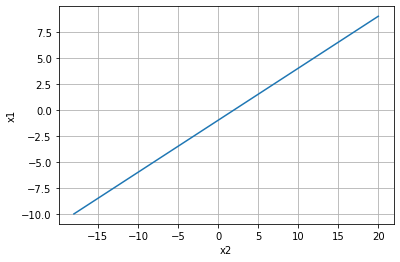
\includegraphics[width=4in]{HW0_plots/hyperplane.png}
    \end{center} 

	\item \points{1} ($n=3$ example) Draw the hyperplane for $w=[1,1,1]^T$, $b=0$? Label your axes. \\
	Following the same principles above $x+y+z=0 \rightarrow z=-x-y$ we have:
	\begin{lstlisting}[language=Python]
import matplotlib.pyplot as plt
from mpl_toolkits import mplot3d
import numpy as np

x2 = np.arange(-10, 10, 1)
x3 = np.arange(-10, 10, 1)
X2, X3 = np.meshgrid(x2, x3)
X1 = -X2 -X3

fg = plt.figure()
ax = plt.axes(projection='3d')
ax.contour3D(X1, X2, X3, 150)
ax.set_zlabel("x3")
ax.set_xlabel("x2")
ax.set_ylabel("x1")
plt.grid()
    \end{lstlisting}
    \begin{center}
    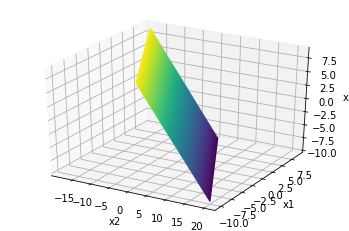
\includegraphics[width=4in]{HW0_plots/hyperplaneB.png}
    \end{center} 

	\item \points{2} Given some $x_0 \in \R^n$, find the \emph{squared distance} to the hyperplane defined by $w^T x + b=0$. In other words, solve the following optimization problem:
	\begin{align*}
	\min_x& \|x_0 - x \|^2\\
	\text{s.t. }&w^Tx +b = 0
	\end{align*}
	(Hint: if $\widetilde{x}_0$ is the minimizer of the above problem, note that $\| x_0 - \widetilde{x}_0 \| = | \frac{w^T(x_0 - \widetilde{x}_0)}{\|w\|} |$. What is $w^T \widetilde{x}_0$?) \\
	    We are looking to minimize the following function: 
	    \begin{align*}
	        f(\vec x) &= \omega^T||\vec x-\vec x_0||^2 + b = 0 \\
	        &= \omega^T||\vec x^T \vec x - 2\vec x\cdot \vec x_0 + \vec x_0^T \vec x_0|| + b \\
	        &= \omega\vec x^T \vec x - 2\omega^T||\vec x\cdot \vec x_0|| + \omega^T\vec x_0^T \vec x_0 + b = 0
	    \end{align*} 
	    Note that values $\vec x^T \vec x$ and $\vec x_0^T \vec x_0$ are just scalars. Minimization can be performed via the method of Lagrange multipliers of the above equation given the constraint that $\vec x$ lies in the plane $\Phi = \omega^T\vec x +b =0$:
	    \begin{align*}
	        \frac{\partial f(\vec x)}{\partial x_i} - \lambda \frac{\partial \Phi(\vec x)}{\partial x_i} &= 0 \\
	        -2\omega^T\frac{\partial ||\vec x\cdot\vec x_0||}{\partial x_i} - \lambda\omega^T \frac{\partial \vec x}{\partial x_i} &= 0 \\
	        -2\omega^T\frac{\partial \vec x}{\partial x_i}\cdot\vec x_0 - \lambda\omega^T\frac{\partial \vec x}{\partial x_i} &= 0 \\
	        \text{\color{red} Following is speculative} \\
	        \left(-2\omega^T\vec x_0 - \lambda\omega^T\right)\frac{\partial \vec x}{\partial x_i} = 0 \\
	    \end{align*}
	    Note that $\omega^T\vec x_0$ is a scalar, that $x_0$ denotes the magnitude of the radius vector of the point we're measuring distance to so it also is a scalar, we can 
\end{enumerate}


\newpage
A.10 For possibly non-symmetric $\mat{A}, \mat{B} \in \R^{n \times n}$ and $c \in \R$, let $f(x, y) = x^T \mat{A} x + y^T \mat{B} x + c$. Define $\nabla_z f(x,y) = \begin{bmatrix} \frac{\partial f(x,y)}{\partial z_1} & \frac{\partial f(x,y)}{\partial z_2} & \dots & \frac{\partial f(x,y)}{\partial z_n} \end{bmatrix}^T$.  


\begin{enumerate}
	\item \points{2} Explicitly write out the function $f(x, y)$ in terms of the components $A_{i,j}$ and $B_{i,j}$ using appropriate summations over the indices.\\
	Not sure what is meant by this but this is how the function would look like written out "explicitly":
	$$
	f(x, y) = 
	\begin{bmatrix} x_1  \\ \vdots \\ x_n \end{bmatrix} \begin{bmatrix} A_{11} & \hdots & A_{1n} \\ \vdots & \ddots & \vdots \\ A_{n1} & \hdots & A_{nn}\end{bmatrix} \begin{bmatrix} x_1  & \hdots & x_n \end{bmatrix} 
	+
	\begin{bmatrix} y_1  \\ \vdots \\ y_n \end{bmatrix} \begin{bmatrix} B_{11} & \hdots & B_{1n} \\ \vdots & \ddots & \vdots \\ B_{n1} & \hdots & B_{nn}\end{bmatrix} \begin{bmatrix} x_1  & \hdots & x_n \end{bmatrix} 
	+
	c \\
	$$
	Writing the above in terms of summations over indices we keep in mind the definition of matrix multiplication: $c_{ij} = \sum_{k=1}^n a_{ik}b_{kj}$. Applied to $Ax$ for example we have $Ax=\sum_{i=1}^n A_{1,i}x_i$. We write the following:
	$$ f(x, y) = \sum_{i=1}^n x_i \sum_{j=1}^n B_{ij}x_j + \sum_{i=1}^n y_i \sum_{j=1}^n B_{ij}x_j + c$$
	
	\item \points{2} What is $\nabla_x f(x,y)$ in terms of the summations over indices \emph{and} vector notation?\\
	In this context $\nabla_x$ represents the gradient operator with respect to elements of vector $x$. In summation form, if coordinates are orthogonal, it's defined as: $\nabla f = \sum_{i=1}^n \, \frac{\partial f}{\partial x^{i}}\frac{1}{h_i}\mathbf{\hat{e}}_i$ where $h$ are the Lame's coefficients (important for coordinate systems except for Cartesian where they're equal to 1) and $x^i$ refers to elements of vector $x$ not exponential operation. Applied to $f(x,y)$:
	$$ \nabla_x f(x, y) = \nabla_x (x^TAx) + \nabla_x (y^TBx) = \frac{\partial}{\partial x_i}\sum_{i=1}^n\sum_{j=1}^n x_iB_{ij}x_j + \frac{\partial}{\partial x_i}\sum_{i=1}^n \sum_{j=1}^n y_iB_{ij}x_j $$
	Apply the chain rule to both elements individually: 
	$$\frac{df(x,y)}{d x} = \frac{\partial f(x,y)}{\partial x} + \dfrac{dy^T(x)}{d x} \frac{\partial (f(x,y))}{\partial y}$$
	\item \points{2} What is $\nabla_y f(x,y)$ in terms of the summations over indices \emph{and} vector notation?
\end{enumerate}

B.2 \points{1} The \textit{trace} of a matrix is the sum of the diagonal entries; $Tr(A) = \sum_i A_{ii}$. If $A\in\mathbb{R}^{n\times m}$ and $B\in\mathbb{R}^{m\times n}$, show that $Tr(AB) = Tr(BA)$.\\
It can be shown in general that trace is invariant under cyclic permutations, which for case of n=2 looks like commutation:
$$\text{tr}(AB)=\sum_i^m (ab)_{ii} = \sum_{i=1}^m\sum_{j=1}^n a_{ij}b_{ji}= \sum_{j=1}^n\sum_{i=1}^m b_{ji}a_{ij} = \sum_i^n (ab)_{jj} = \text{tr}(BA)$$
using the fact that product of $n\times m$ and $m\times n$ matrix is an $m\times m$ matrix and that the trace of a square matrix can be rewritten as:
$$\text{tr}(A^TB)=\sum_{i,j}A_{ij}B_{ij}$$
as per Wikipedia.\\

B.3 \points{1} Let $v_1,\dots,v_n$ be a set of non-zero vectors in $\mathbb{R}^d$. Let $V = [v_1,\dots,v_n]$ be the vectors concatenated. 
    \begin{enumerate}
        \item What is the minimum and maximum rank of $\sum_{i=1}^n v_i v_i^T$? \\
        Basis of an $\mathbb{R}^d$ is spanned by $d$ linearly independent vectors. So the maximum rank of a matrix will be d. Minimal rank of a matrix would always be 0 in case of a zero matrix, but since the vectors $v$ must be non-zero the minimal rank of V would be 1 in the case all $v$ are the same unit vectors. 
        \item What is the minimum and maximum rank of $V$? \\
        Same as a) (are these supposed to be like trick questions?)
        \item Let $A \in \mathbb{R}^{D \times d}$ for $D > d$. What is the minimum and maximum rank of $\sum_{i=1}^n (A v_i) (A v_i)^T$?
        \item What is the minimum and maximum rank of $AV$? What if $V$ is rank $d$?
    \end{enumerate}

\section*{Programming}

A.11 For the $A, b, c$ as defined in Problem 8, use
  NumPy to compute (take a screen shot of your answer):
  \begin{enumerate}
  \item \points{2} What is $A^{-1}$?
  \item \points{1} What is $A^{-1}b$? What is $Ac$?
  \end{enumerate}  
  
    \begin{center}
    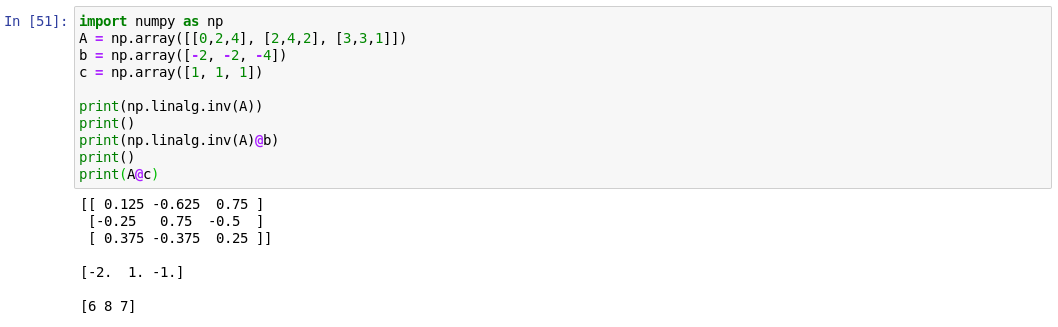
\includegraphics[width=4in]{HW0_plots/numpy.png}
    \end{center} 


A.12 \points{4} Two random variables $X$ and $Y$ have equal
  distributions if their CDFs, $F_X$ and $F_Y$, respectively, are
  equal, i.e. for all $x$, $ |F_X(x) - F_Y(x)| = 0$. 
The central limit theorem says that the sum of $k$ independent,
zero-mean, variance-$1/k$ random variables converges to a (standard) Normal distribution as $k$ goes off to infinity.  
We will study this phenomenon empirically (you will use the Python packages Numpy and Matplotlib). 
Define $Y^{(k)} = \frac{1}{\sqrt{k}} \sum_{i=1}^k B_i$ where each $B_i$ is equal to $-1$ and $1$ with equal probability.
From your solution to problem 5, we know that $\frac{1}{\sqrt{k}} B_i$ is zero-mean and has variance $1/k$.
\begin{enumerate}
\item For $i=1,\dots,n$ let $Z_i \sim \mathcal{N}(0,1)$. If $F(x)$ is the true CDF from which each $Z_i$ is drawn (i.e., Gaussian) and $\widehat{F}_n(x) = \frac{1}{n} \sum_{i=1}^n \1\{ Z_i \leq x)$, use the answer to problem 1.5 above to choose$n$ large enough such that, for all $x \in \R$, $ \sqrt{\E[(\widehat{F}_n(x)-F(x))^2 ]} \leq 0.0025$, and plot $\widehat{F}_n(x)$ from $-3$ to $3$. \\(Hint: use \texttt{Z=numpy.random.randn(n)} to generate the random variables, and \texttt{import matplotlib.pyplot as plt}; \texttt{plt.step(sorted(Z), np.arange(1,n+1)/float(n))} to plot). 
	\begin{lstlisting}[language=Python]
import matplotlib.pyplot as plt
import numpy as np

n = 20000
Z = np.sign(np.random.randn(n))
plt.step(sorted(Z), np.arange(1, n + 1) / float(n))

plt.xlim(-3, 3)
plt.xlabel("Observations")
plt.ylabel("Probability")
plt.show()
    \end{lstlisting}
    \begin{center}
    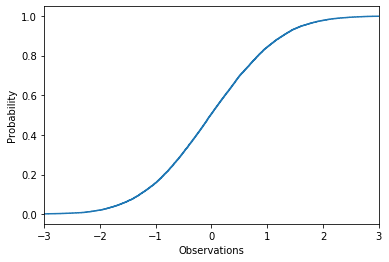
\includegraphics[width=4in]{HW0_plots/cumdist1.png}
    \end{center} 
\item For each $k \in \{1, 8, 64, 512\}$ generate $n$ independent copies $Y^{(k)}$ and plot their empirical CDF on the same plot as part a.\\ (Hint: $\texttt{np.sum(np.sign(np.random.randn(n, k))*np.sqrt(1./k), axis=1)}$ generates $n$ of the $Y^{(k)}$ random variables.) 
	\begin{lstlisting}[language=Python]
import matplotlib.pyplot as plt
import numpy as np

def Yk(n, k=1):
    """Returns and array of samples of function:
    
        Y^{(k)} = 1/sqrt(k) \sum_1^k B_i
    
    where B_i = +1 or +1 with equal probablility. 
    
    Parameters
    -----------
    n : `int`
        Number of samples of Y^(k). 
    k : `int`
        Upper bound of the Y^(k) sum
    """
    B = np.sign(np.random.randn(n, k))
    return np.sum(np.sqrt(1.0/k)*B, axis=1)


n = 20000
for k in [1, 8, 64, 512]:
    Y = Yk(n, k)
    plt.step(sorted(Y), np.arange(1, n + 1) / float(n), label='{0}'.format(k))

gaus = np.random.normal(size=n)
plt.step(sorted(gaus), np.arange(1, n + 1) / float(n), label='Gaussian')    

plt.legend()
plt.xlim(-3, 3)
plt.xlabel("Observations")
plt.ylabel("Probability")
plt.show()
    \end{lstlisting}
    \begin{center}
    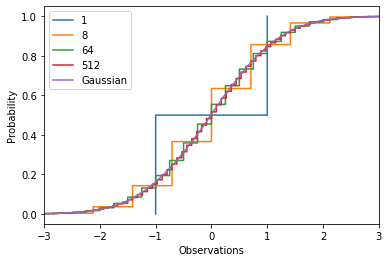
\includegraphics[width=4in]{HW0_plots/cumdist2.png}
    \end{center} 

\end{enumerate}
\end{document}
